% This text is proprietary.
% It's a part of presentation made by myself.
% It may not used commercial.
% The noncommercial use such as private and study is free
% Sep. 2005 
% Author: Sascha Frank 
% University Freiburg 
% www.informatik.uni-freiburg.de/~frank/
%
% additional usepackage{beamerthemeshadow} is used
%  
%  \beamersetuncovermixins{\opaqueness<1>{25}}{\opaqueness<2->{15}}
%  with this the elements which were coming soon were only hinted
\documentclass{beamer}
\usepackage{beamerthemeshadow}
\usepackage{graphicx}
\usepackage{hyperref}
\usepackage{amsmath}
\usepackage{amssymb}
\hypersetup{
    colorlinks=true,
    linkcolor=blue,
    filecolor=magenta,      
    urlcolor=cyan,
}
\begin{document}
\title{2D $\phi^4$ theory: A study in OpenACC with PGI++}  
\author{Dean Howarth}
\date{\today} 

\frame{\titlepage} 

\frame{\frametitle{Table of contents}\tableofcontents} 

\section{Introduction} 
\frame{\frametitle{Coming up...}
\begin{enumerate}
\item We need a concrete physical model to use: 2D $\phi^4$
\item Within the 2D $\phi^4$ code are some important algorithms (HMC, cluster decomposition)
\item Identify opportunities for parallelism
\item Use OpenACC and pgi++ to exploit those opportunities.
\item Inspect our optimisations using profiling tools, gain insights into further progress
\item Apply all of the above to an different code.
\end{enumerate}\
}

\section{2D $\phi^4$ theory and its discrete analogue (Lecture)} 
\frame{\frametitle{Why study 2D $\phi^4$ theory?}
\begin{enumerate}
\item We know all the answers! Same universality class as 2D Ising model
\item Contains most of the ingredients required for computational physics problems
\begin{enumerate}
\item Boundary conditions (periodic)
\item A differential operator
\item Markov chain dynamics
\end{enumerate}
\item We don't actually know all the answers... (Google "2D $\phi^4$ " for recent results)
\begin{enumerate}
\item Long range coupling still an \href{https://arxiv.org/pdf/1703.05325.pdf}{ongoing debate} 
\item Add one more dimension, you're in \href{https://en.wikipedia.org/wiki/Ising_critical_exponents}{unknown territory}
\end{enumerate}
\end{enumerate}\
}

\frame{\frametitle{Path Integrals: A lightning tour}
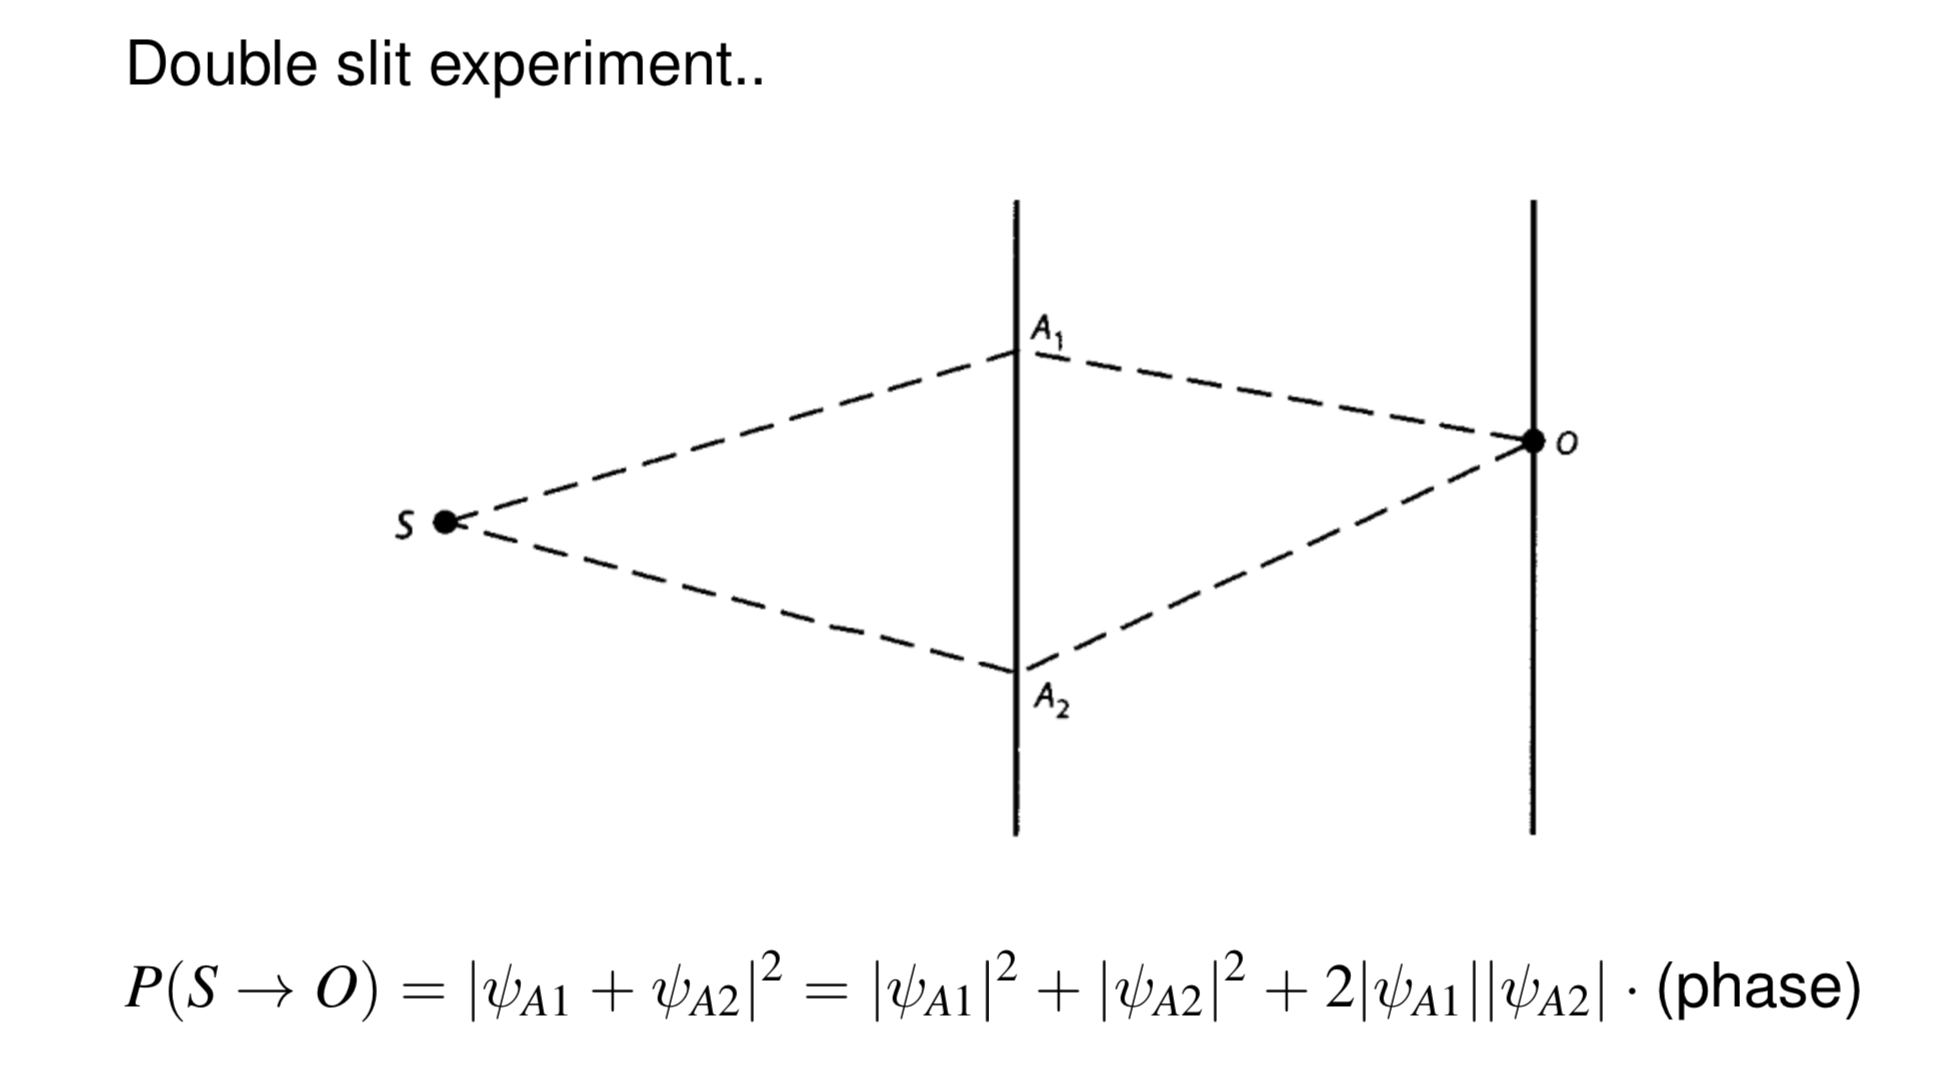
\includegraphics[width=1.0\columnwidth]{path1}
}

\frame{\frametitle{Path Integrals: A lightning tour}
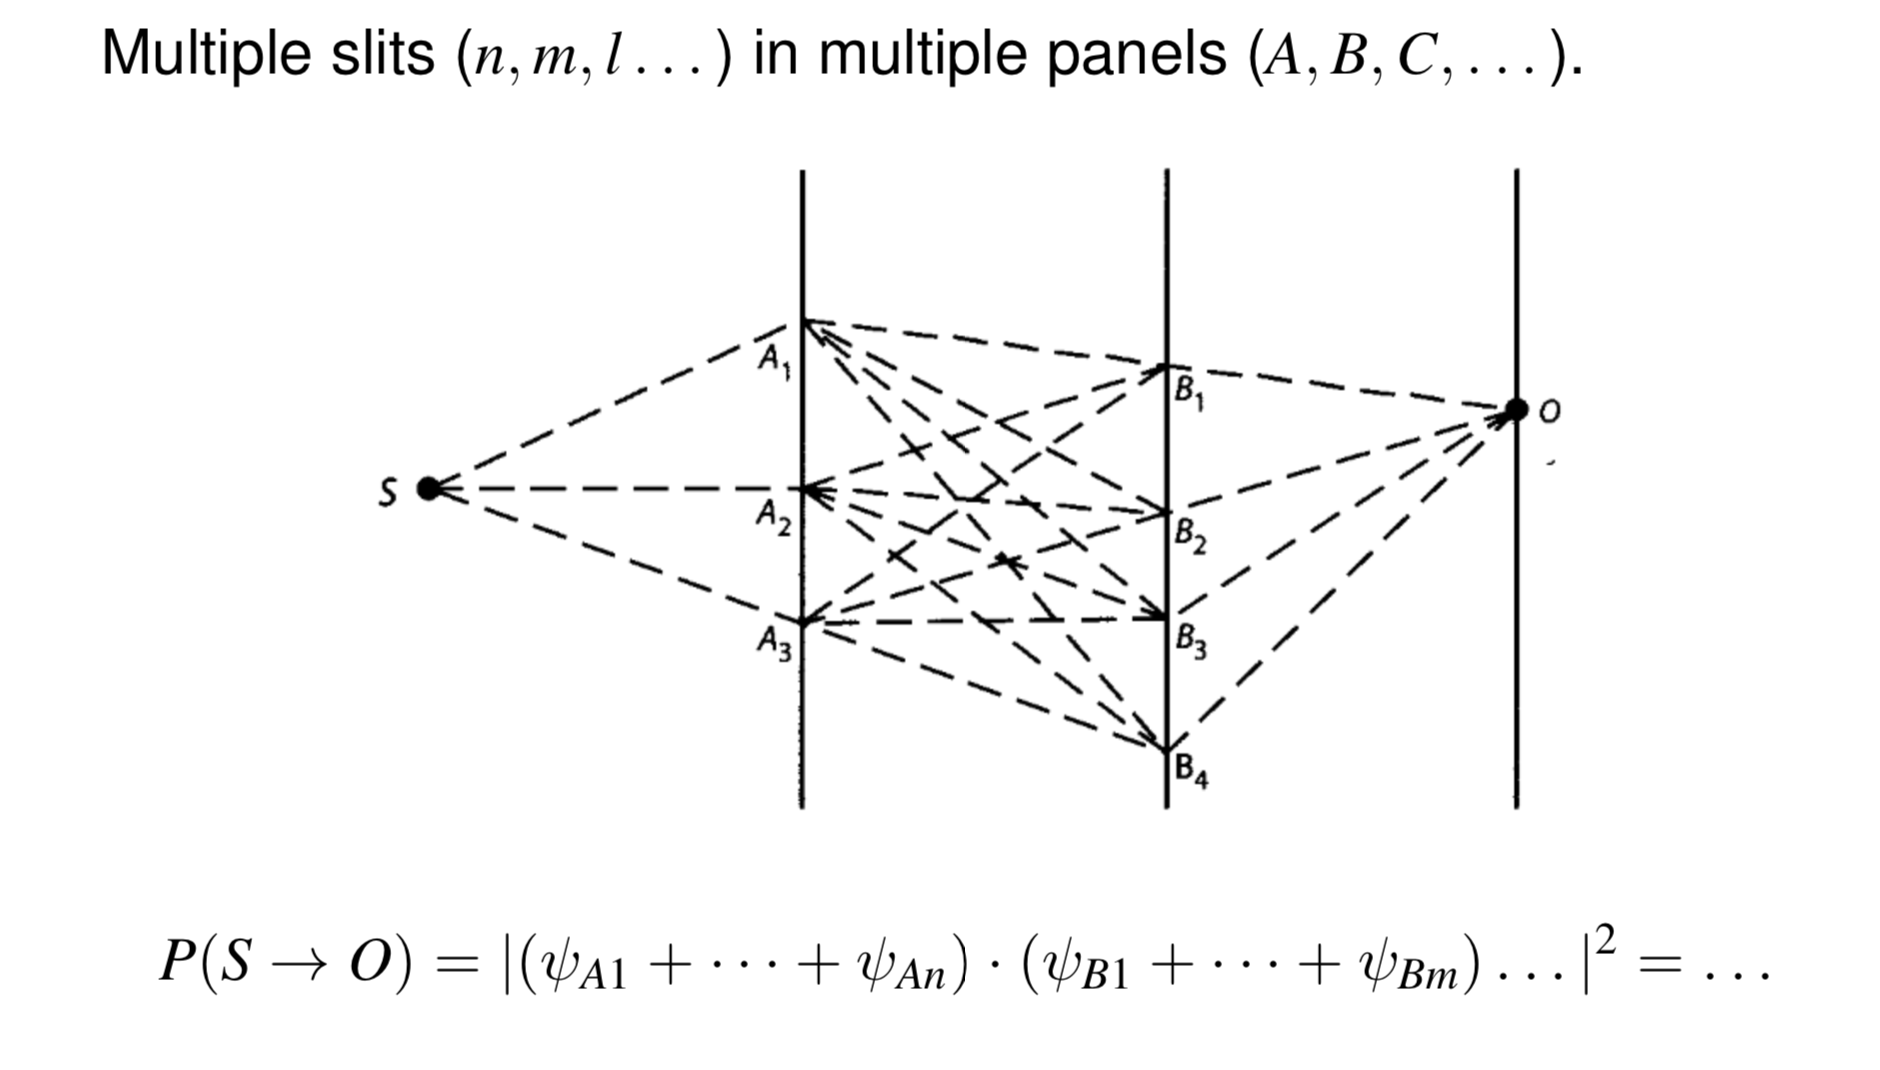
\includegraphics[width=1.0\columnwidth]{path2}
}

\frame{\frametitle{Path Integrals: A lightning tour}
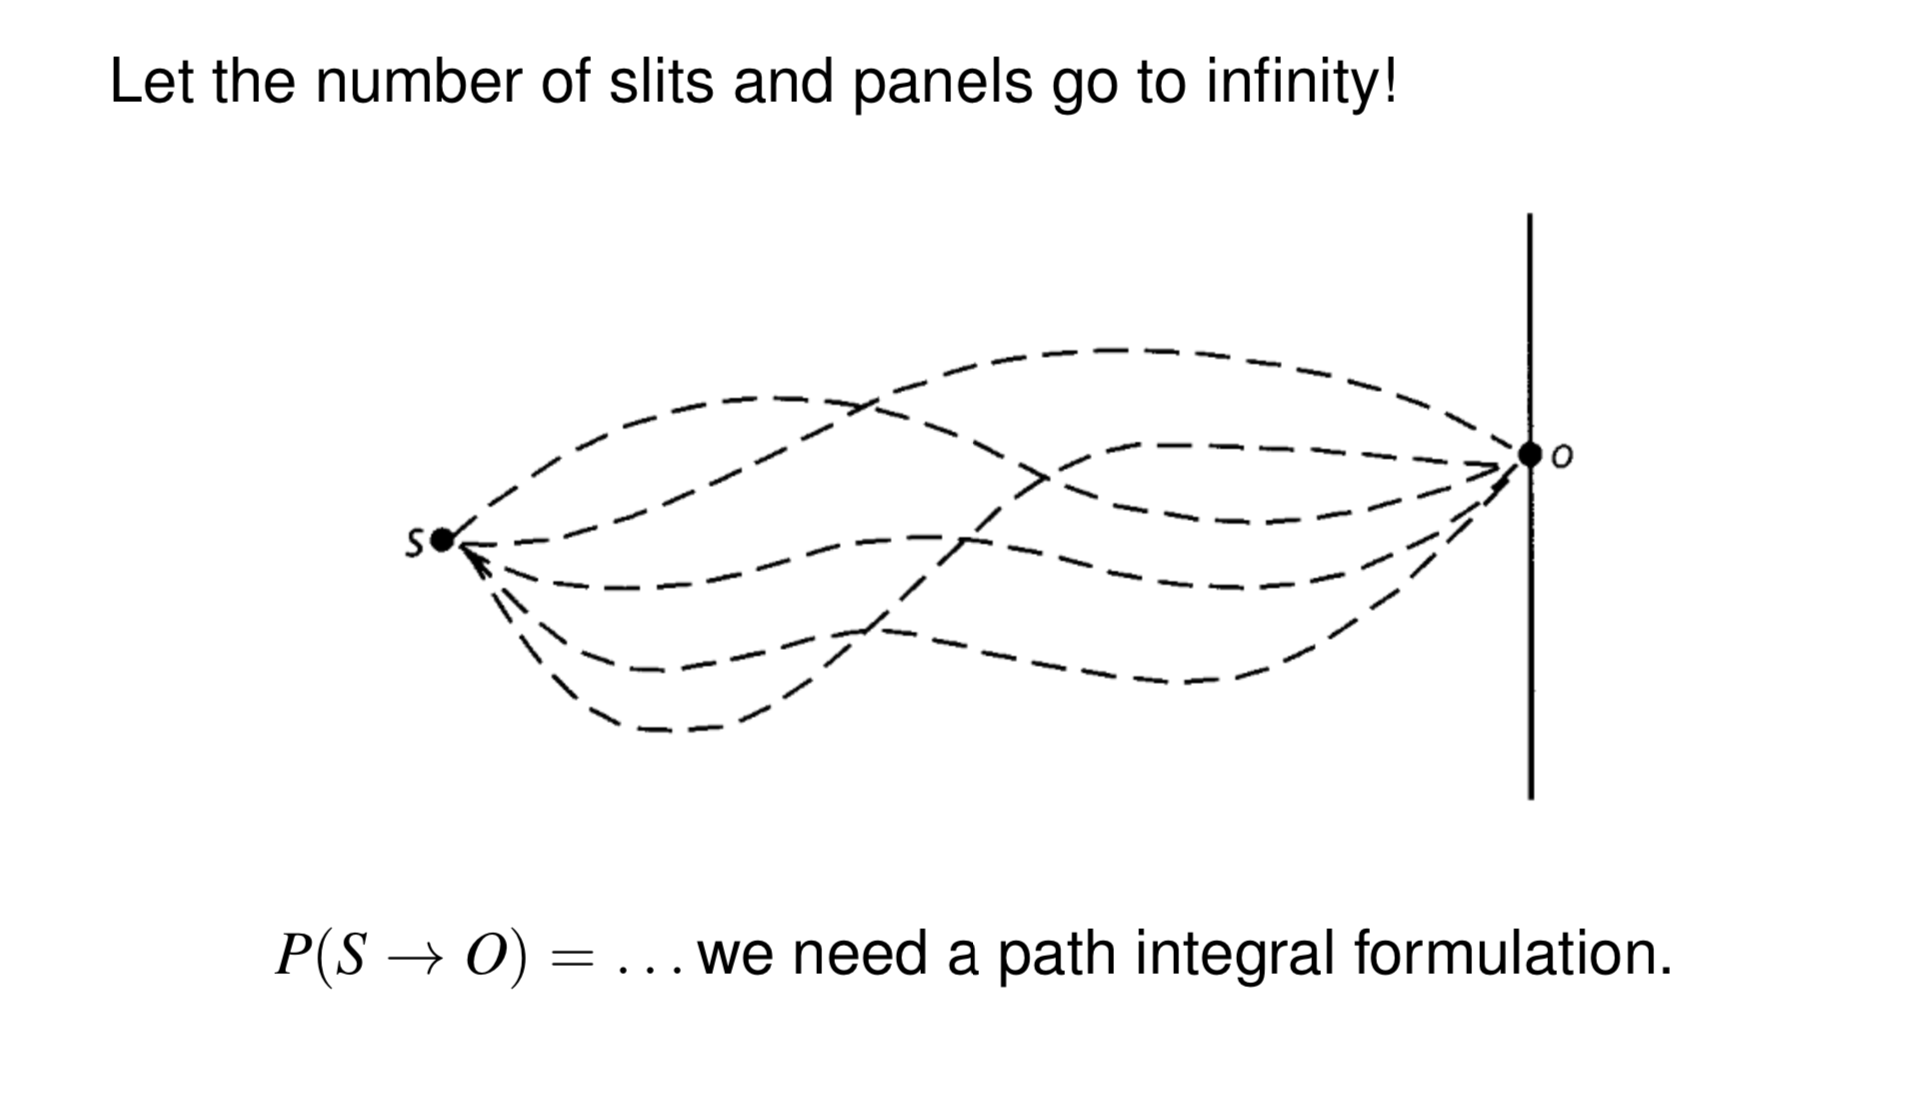
\includegraphics[width=1.0\columnwidth]{path3}
}

\frame{\frametitle{Path Integrals: A lightning tour}
Each path contributes an amplitude (weight) to the final answer. The further away from the classical path, the less weight is given to the path. These weights are given by a path integral.
\begin{align}
\langle \phi^2\rangle&=\frac{\int D\phi exp(iS[\phi])\phi^2}{\int D\phi exp(iS[\phi])}\nonumber
\end{align}
where
\begin{align}
S(\phi)&=\int dx^2 \mathcal{L}(x)\nonumber\\
\mathcal{L}(x)&=\frac{1}{2}(\nabla\phi(x))^2 - \frac{1}{2}m^2\phi^2(x) - \frac{1}{4!}\lambda\phi^4(x)\quad x=(x,t)\nonumber
\end{align}
}

\frame{\frametitle{Markov Chains}
What happens when one can't solve the path integral? How does one simulate a quantum field theory? Probabilistically.\\
\vspace{5mm}
Quantum fields are superpositions of classical field configurations. If we can identify a representative sample of those configurations, we will be able to to compute a good estimate of an expectation value.\\
{\bf This is in perfect analogy with statistical sampling: a robust estimate of the mean of a data set can be obtained via an unbiased sample from that data set.}\\
\vspace{5mm}
Markov chains offer us the ability to create such a sample. But first, we must discretise.
}

\frame{\frametitle{Discretising the Lagrangian}
The continuum 2D $\phi^4$ {\bf Minkowski} Lagrangian
\begin{align}
\mathcal{L}(x)&=\frac{1}{2}(\nabla\phi(x))^2 - \frac{1}{2}m^2\phi^2(x) - \frac{1}{4!}\lambda\phi^4(x)\quad x=(x,t)
\end{align}
The discrete 2D $\phi^4$ {\bf Euclidean} Lagrangian
\begin{align}
\mathcal{L}_E(x)=&\frac{1}{2}[(\phi(x+an_x) - \phi(x))^2 + (\phi(x+an_y) - \phi(x))^2]\\\nonumber
&+ \frac{1}{2}m^2\phi^2(x) + \frac{1}{4!}\lambda\phi^4(x)\quad x=(x,y)
\end{align}
Discretisation of the differential operator introduces errors. Can you work out what those errors are? (see me during the break)
}

\frame{\frametitle{Discretising the Lagrangian}
\center 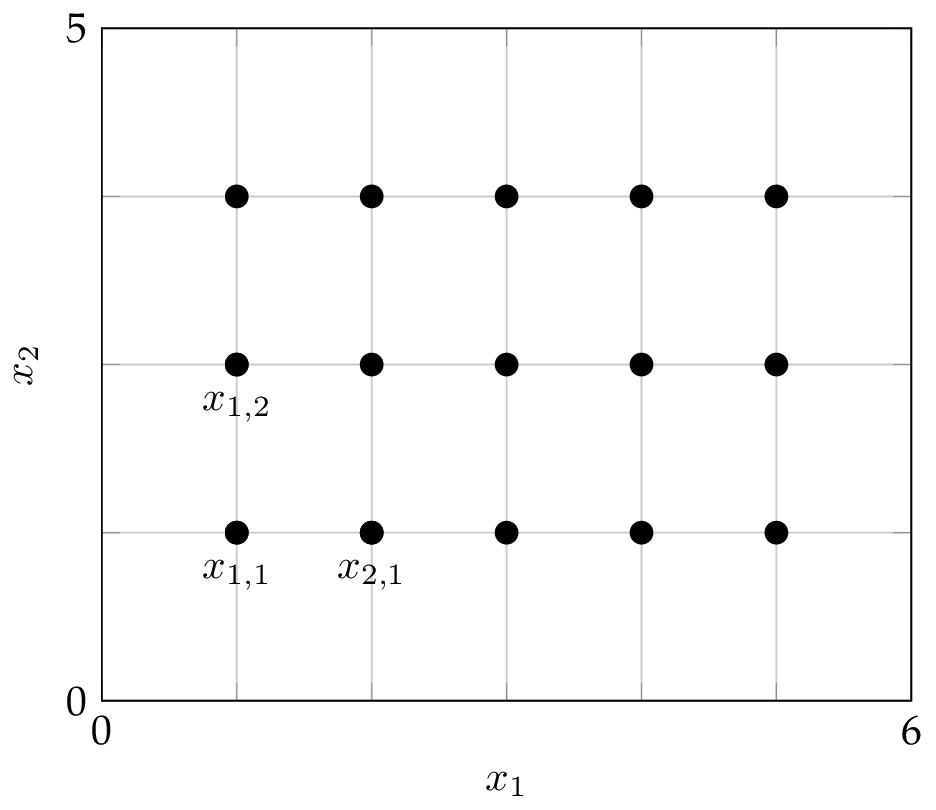
\includegraphics[width=0.75\columnwidth]{discrete-laplacian-2D-grid.png}
}

\frame{\frametitle{Hybrid Monte-Carlo and Importance sampling}
If you Google "Hybrid Monte-Carlo and Importance sampling" you will be occupied for weeks! For now, you only need to understand the concepts.
\begin{itemize}
\item Wick Rotation: rotate the $t$-dimension to $-it$
\begin{align}
\langle \phi^2\rangle_E&=\frac{\int D\phi exp(-S_E[\phi])\phi^2}{\int D\phi exp(-S_E[\phi])}\nonumber
\end{align}
\item Fictitious momenta: noise with zero mean
\begin{align}
\langle \phi^2\rangle_E&=\frac{\int D\phi exp(-\frac{1}{2}\pi^2-S_E[\phi])\phi^2}{\int D\phi exp(-\frac{1}{2}]\pi^2-S_E[\phi])}\nonumber
\end{align}
\item Fictitious hamiltonian: field evolution through an extra dimension
\begin{align}
\mathcal{H}_E(P,\phi)=\frac{1}{2}\pi^2+S_E[\phi]\nonumber
\end{align}
\end{itemize}
}

\frame{\frametitle{Hybrid Monte-Carlo and Importance sampling}
We evolve the $\phi$ field through a fictitious time variable $\tau$ using the Hamiltonian equations of motion.
\begin{align}
\frac{\partial \phi}{\partial \tau}&=\frac{\partial\mathcal{H}}{\partial \pi},\quad \frac{\partial \pi}{\partial \tau}=-\frac{\partial\mathcal{H}}{\partial \phi}=-\frac{\partial S}{\partial \phi}
\end{align}
We can solve these equations (evolve the $\phi$ field) using Leapfrog algorithm (See phi4Serial.cpp and Stefan's notes). We can explore the phase space further using cluster algorithms. (See WolffCluster.pdf for more details)
}

\frame{\frametitle{The HMC algorithm for $phi^4$ theory}
Here is the HMC, with annotations (search for 'Step n:') directing you to the relevant code in phi4Serial.cpp
\begin{itemize}
\item Step1: choose gaussian distributed momenta $P_i \in exp(-\pi^2_i/2)$
\item Step2: evolve the $\phi$ and $\pi$ fields to candidate configurations $\phi'$ and $\pi'$:
\begin{align}
\frac{d}{d \tau}\phi_x(\tau) &= \frac{\partial}{\partial \pi_x}\mathcal{H}(\pi(\tau), \phi(\tau))\nonumber\\
\frac{d}{d \tau}\pi_x(\tau) &=-\frac{\partial}{\partial \phi_x}\mathcal{H}(\pi(\tau), \phi(\tau))\nonumber
\end{align}
\item Step3: accept candidate configurations with probability
\begin{align}
P_{accept} = min(1,\exp(-(\mathcal{H}' - \mathcal{H})))\nonumber
\end{align}
\end{itemize}
}

\frame{\frametitle{The HMC algorithm for $phi^4$ theory}
Step 2 in a bit more detail.  (search for 'Step 2.n:')
\begin{itemize}
\item Step 2.1: $\pi_{1/2} = \pi_0 - \frac{d\tau}{2}F(\phi)$
\item Step 2.2: For $k=1...n-1$
\begin{align}
\phi_{k} &= \phi_{k-1} + \pi_{k-1/2}d\tau\nonumber\\
\pi_{k+\frac{1}{2}} &= \pi_{k-\frac{1}{2}} - F(\phi)d\tau\nonumber
\end{align}
\item Step 2.3: $\phi_{n} = \phi_{n-1} + \pi_{n-\frac{1}{2}}d\tau$
\end{itemize}
$F(\phi) = \nabla S(\phi)$ is a fictitious force, driven by the `action potential'.
}

\frame{\frametitle{The HMC algorithm for $phi^4$ theory}
This is why the velocity Verlet algorithm is often called Leapfrog...
\center 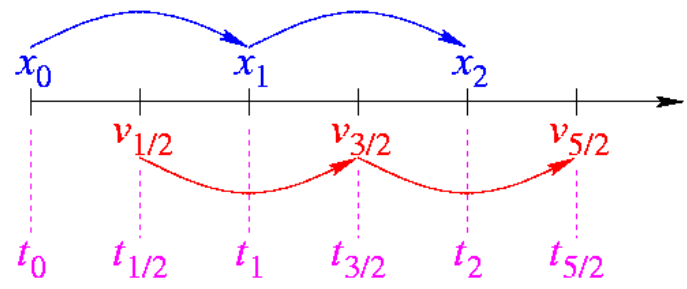
\includegraphics[angle=0, width=1.0\columnwidth]{leapfrogMethod.png}
}

\frame{\frametitle{The HMC algorithm for $phi^4$ theory}
This is why the we call it the `action potential'...
\center 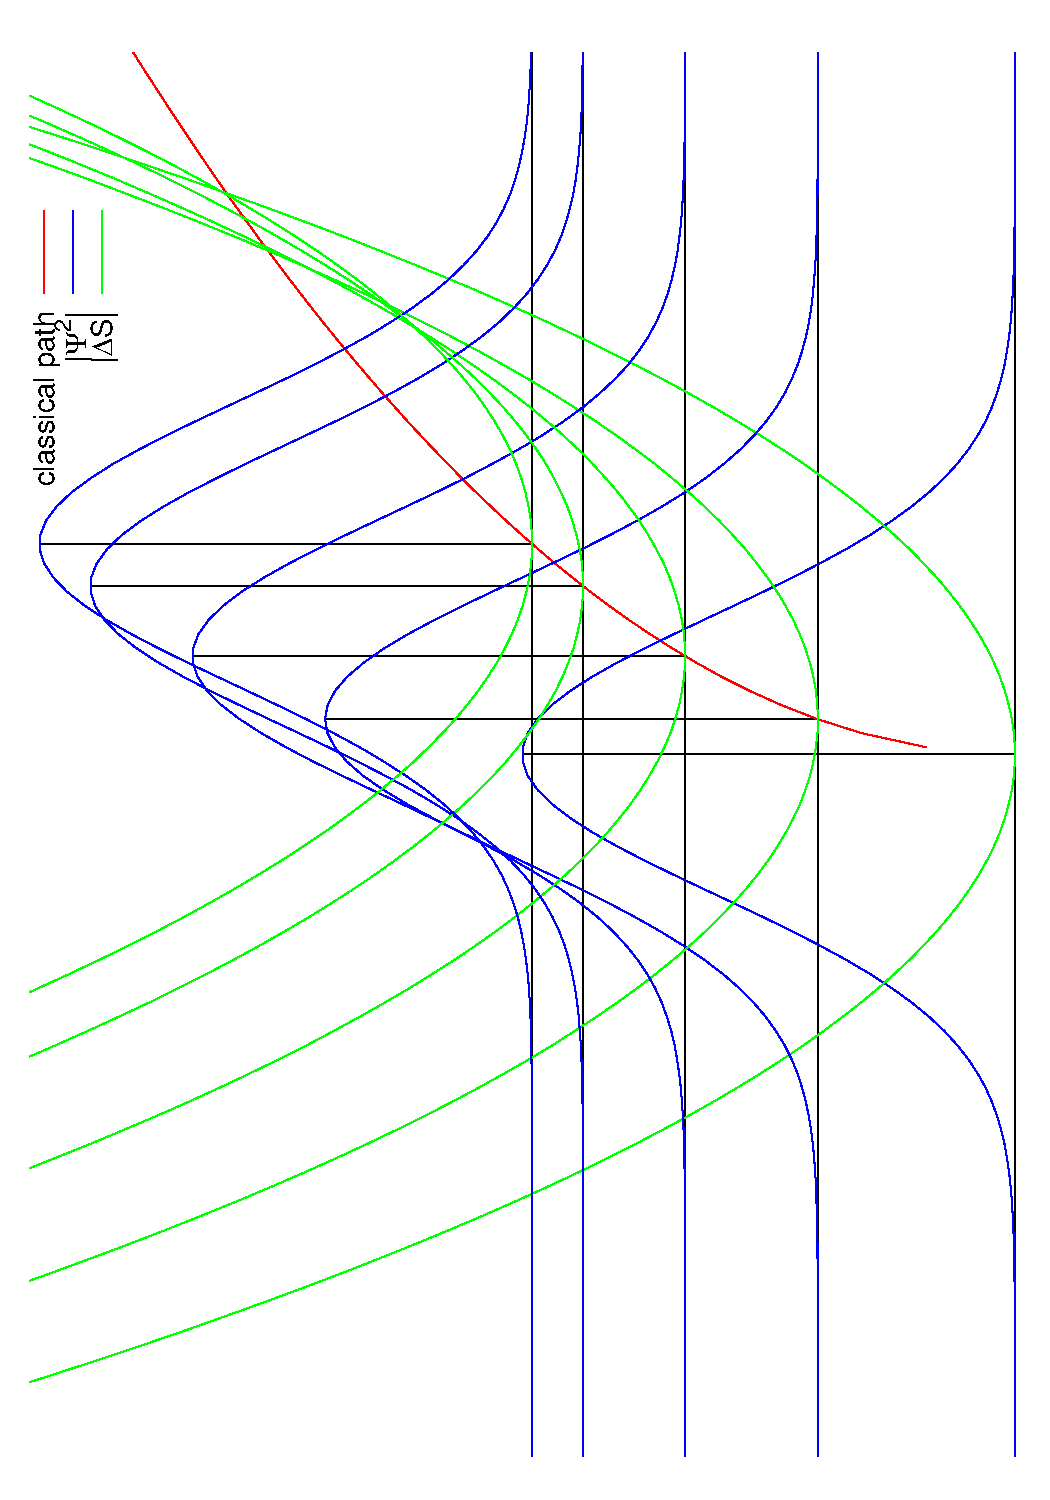
\includegraphics[angle=270, width=0.75\columnwidth]{classical-action.pdf}
}

\frame{\frametitle{HMC is its own thang}
\center 
\includegraphics[width=0.50\columnwidth]{anyQuestions}
}

\frame{\frametitle{Cluster Algorithms}
Cluster decomposition of $\phi^4$ theory can lead to some staggeringly efficient evolution algorithms. It was pioneered by Fortuin and Kasteleyn in the late 60s. Omitting the gory details, one can write the partition function of a lattice theory as the sum of all possible clusters. One constructs such clusters with a probability,
\begin{align}
P[bond(x,y)]&=1-\exp(-2\phi(x)\phi(y))
\end{align}
Swendsen and Wang used this result to produce an algorithm that, without rejection, moves a lattice from one configuration to another. Ulli Wolff came up with one too.
}

\frame{\frametitle{Swendsen-Wang And Wolff}
Swendsen-Wang:
\begin{itemize}
\item Step 1: Test every n.n. bond ONCE to see if they are connected via a bond using $P[bond(x,y)]=1-\exp(-2\phi(x)\phi(y))$
\item Step 2: Identify every connected cluster on the lattice.
\item Step 3: Flip each cluster with 50\% probability.
\end{itemize}
Wolff:
\begin{itemize}
\item Step 1: Choose a lattice site at random.
\item Step 2: Identify every site connected to that original site using $P[bond(x,y)]=1-\exp(-2\phi(x)\phi(y))$
\item Step 3: Flip the cluster with 100\% probability.
\end{itemize}
You have been provided with notes on the Wolff algorithm, and code for the Swendsen-Wang. Can you write a Wolff cluster algorithm in the activity time?
}

\section{2D $\phi^4$ with PGI++ (Code Review)} 
\frame{\frametitle{The serial implementation} 
Provided under\\{\fontfamily{<pcr>}\selectfont RPI-Advanced-Cyberinfrastructure/phi4AndOpenACC/phi4Serial}\\
is a set of routines that perform HMC on a $\phi^4$ theory. Let's read through the code and understand it before using PGI++.\\
Points to consider:\\
\begin{itemize}
\item HMC is performed once for multiple cluster updates... why?
\item Can you decipher what the cluster algorithm does?
\item The {\fontfamily{<courier>}\selectfont trajectory()} function performs the Leapfrog integration. Can you see how it does it?
\item Looking ahead, can you intuitively see where the routines can be easily parallelised?
\end{itemize}
}

\frame{\frametitle{What are OpenACC and PGI++?}
PGI++ is an OpenACC compiler. It is able to compile C++ standard code, along with OpenACC compliant pragmas:
\center{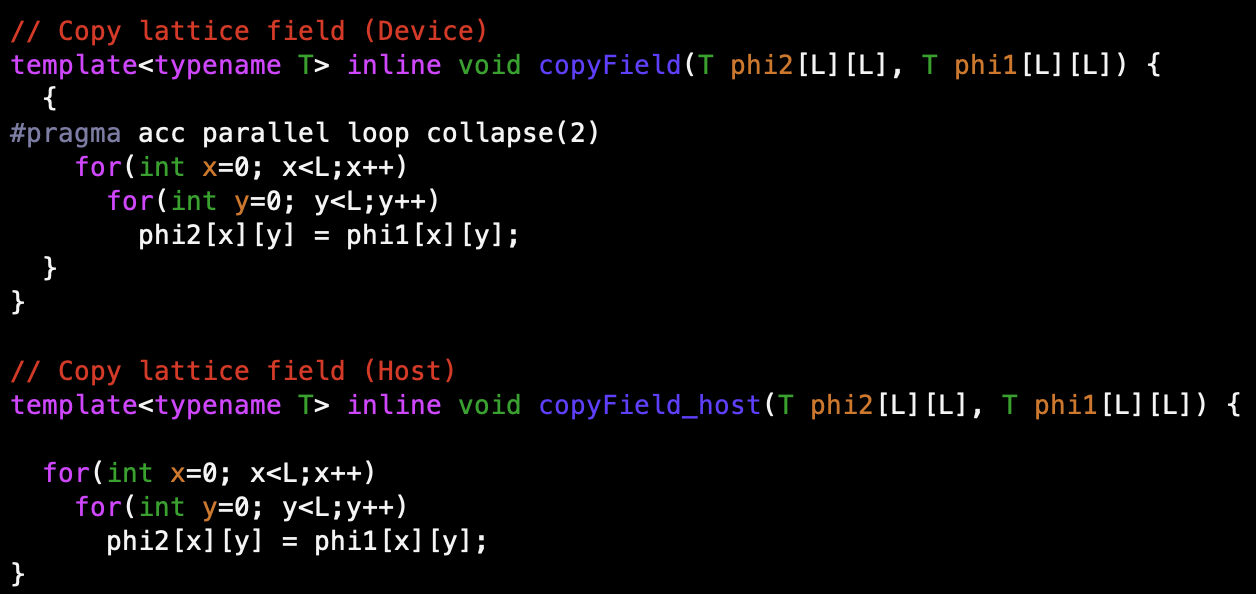
\includegraphics[width=0.75\columnwidth]{examplePragma}}\\
A pragma is a `hint' or `directive' to the compiler. In the above excerpt, we have informed the compiler that the (2) nested loop may be collapsed. I.e., each iteration is independent. 
}

\frame{\frametitle{Using OpenACC and PGI++}
We are going to learn OpenACC by example. Having seen and understood some serial code, we shall add OpenACC pragmas where relevant and explain each addition in context.
\begin{itemize}
\item v0: The serial code, with timings.
\item v1: Lots of OpenACC additions to the HMC.
\item v2: More OpenACC in the cluster decomposition.
{\center ACTIVITY CHALLENGES}
\item v3: Can you write a Wolff algorithm? Can you make the HMC more efficient? Can you write a two-point correlation function measurement $\langle \phi(x)\phi(y) \rangle$ and make it run at nosebleed speed?
\center{Ask questions, work in groups, read the code comments, happy hacking!}
\end{itemize}
}

\end{document}






















